\section{Database caching}

WordPress was programmed with the support of database caching in mind. Core functions and methods querying the database (such as get\_option, get\_posts and others) use WordPress Object Cache API \cite{WP:Object-Cache-API} on the background. \\

The default Object Cache API caches the database queries and results in a PHP array, thus only for a duration of the script execution (one request). On one hand, this mechanism is useful in templates, where the same information about the site is retrieved multiple times (for example get\_bloginfo function). On the other hand, when many users visiting our site request the same page, the same database queries have to be made unnecessarily multiple times. \\

If we need to store the database cache persistently, we can use an in-memory database. "An in-memory database is a database management system that primarily relies on main memory for computer data storage. It is contrasted with database management systems that employ a disk storage mechanism. Main memory databases are faster than disk-optimized databases since the internal optimization algorithms are simpler and execute fewer CPU instructions. Accessing data in memory eliminates seek time when querying the data, which provides faster and more predictable performance than disk." \cite{Wiki:in-memory-database}\\

The two most popular in-memory databases in the WordPress ecosystem are Memcached and Redis. In our work we have chosen to work with Redis as it is modern, well-supported and having all the features of Memcached. \cite{SO:Redis-vs-Memcached} In order for WordPress Object Cache API to use Redis for database caching, we need to install Redis server and Redis PHP connector (driver). We have prepared an Ansible playbook which downloads a PHP driver for Redis and installs it into the currently installed WordPress site (whether basic or advanced). Within your command line, navigate to the wordpress-ansible directory and run the "wordpress\_redis\_db\_cache.yml" Ansible playbook:

\begin{lstlisting}
ansible-playbook -i hosts wordpress\_redis\_db\_cache.yml
\end{lstlisting}

Analogous to how we benchmarked the web-serving software in the previous section, we configured a Loader.io test and performed several load tests for the site with Redis database caching enabled. Suprisingly, resulting charts did not show any noticeable improvements \cite{Loader.io:nginx_hhvm_redis} over the other tests. Contemplating over this issue, we think that the database on our testing server is not a bottleneck. However, as this has not been proved yet, it might be a subject of a future work.

\section{Page caching} \label{page-caching}

Page caching is storing the output of a PHP interpreter (such as PHP-FPM or HHVM) on a disk or in RAM on the first request to a page (URL) and serving this stored (cached) content on subsequent ones. Page caching increses the performance of a web server considerably. To put it in simplistic terms, page caching converts a dynamic website into a static one. The most noticeable downside of page caching is that it is hard, if not impossible, to cache highly dynamic pages like constantly changing homepage or user profile page. In such circumstances, it is usually better to bypass the caching mechanisms and process the request with a PHP interpereter. \\

The easiest (but not the most performant) way to achieve page caching in WordPress-based site is to use a plugin such as W3 Total Cache or WP Super Cache. These plugins store a page on your server's disk as an HTML file. When the page is requested for the second time, the HTML file is sent back as a response without having to process it within WordPress, thus saving hundreds to thousands of milliseconds. The largest advantages of these plugins are their ease-of-use. They usually come with simple user interface and a mechanism to bypass the cache for logged in users and highly dynamic pages. It is also quite straightforward to purge the cache if a new piece of content has been added with most of the plugins doing it automatically. \\

However, we prefer to set up page caching at a lower level, directly in Nginx. Nginx FastCGI module \cite{Nginx:FastCGI-module} includes a caching mechanism. The advantages of this approach are that the content is stored in RAM (as opposed to a disk) and with the use of various Nginx directives \cite{Nginx:directives}, we get a fine-grained control over the caching process. What is more, there is a plugin called Nginx Helper, which is able to clear the cache when a new WordPress post or page is added. In our work, we have used Nginx's FastCGI cache to increase the server's web-serving performance. \\

We are going to benchmark the performance of our testing server with Nginx FastCGI caching enabled. Create a new Loader.io test with a duration of 15 seconds, maintaining client load from 300 to 1000 simultaneous clients to the root of our WordPress-powered site. \cite{Loader.io:nginx_hhvm_fastcgi_caching} To configure the FastCGI caching, within your command line, navigate to the wordpress-ansible directory and run the "nginx\_hhvm\_fastcgi\_cache.yml" Ansible playbook:

\begin{lstlisting}
ansible-playbook -i hosts nginx_hhvm_fastcgi_cache.yml
\end{lstlisting}

The resulting clients versus average response time chart can be observed on the figure \ref{fig:nginx_fastcgi_caching}. Note that we did a manual request (non-cached one) before starting the test for Nginx to cache it.

\begin{figure}[H]
\begin{center}
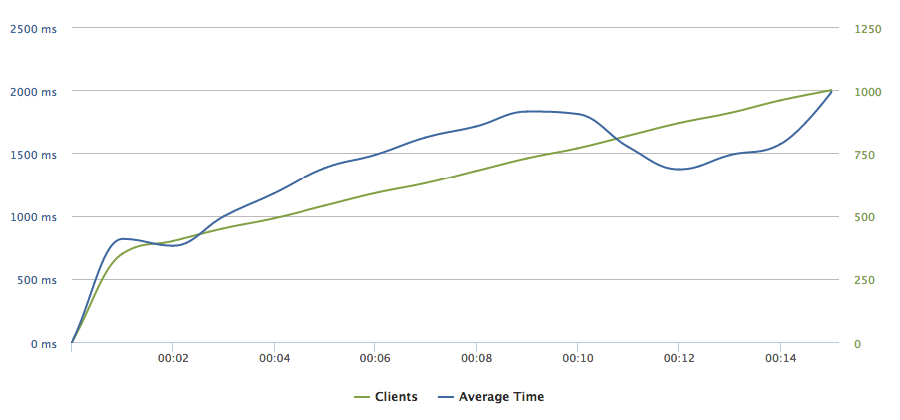
\includegraphics[scale=0.5]{figures/Nginx_FastCGI_caching.png}
\caption{Nginx with FastCGI caching: clients versus average response time}
\label{fig:nginx_fastcgi_caching}
\end{center}
\end{figure}

With our three CPU testing server, we were able to serve 1000 concurrent requests while maintaining the average response time under 2000 ms. Compare it with the previous testing \ref{advanced-wordpress-hhvm}, where we barely served 200 concurrent requests under 8000 ms average response time. Another interesting statistic is the output of Htop process viewer, which can be observed on the figure below.

\begin{figure}[H]
\begin{center}
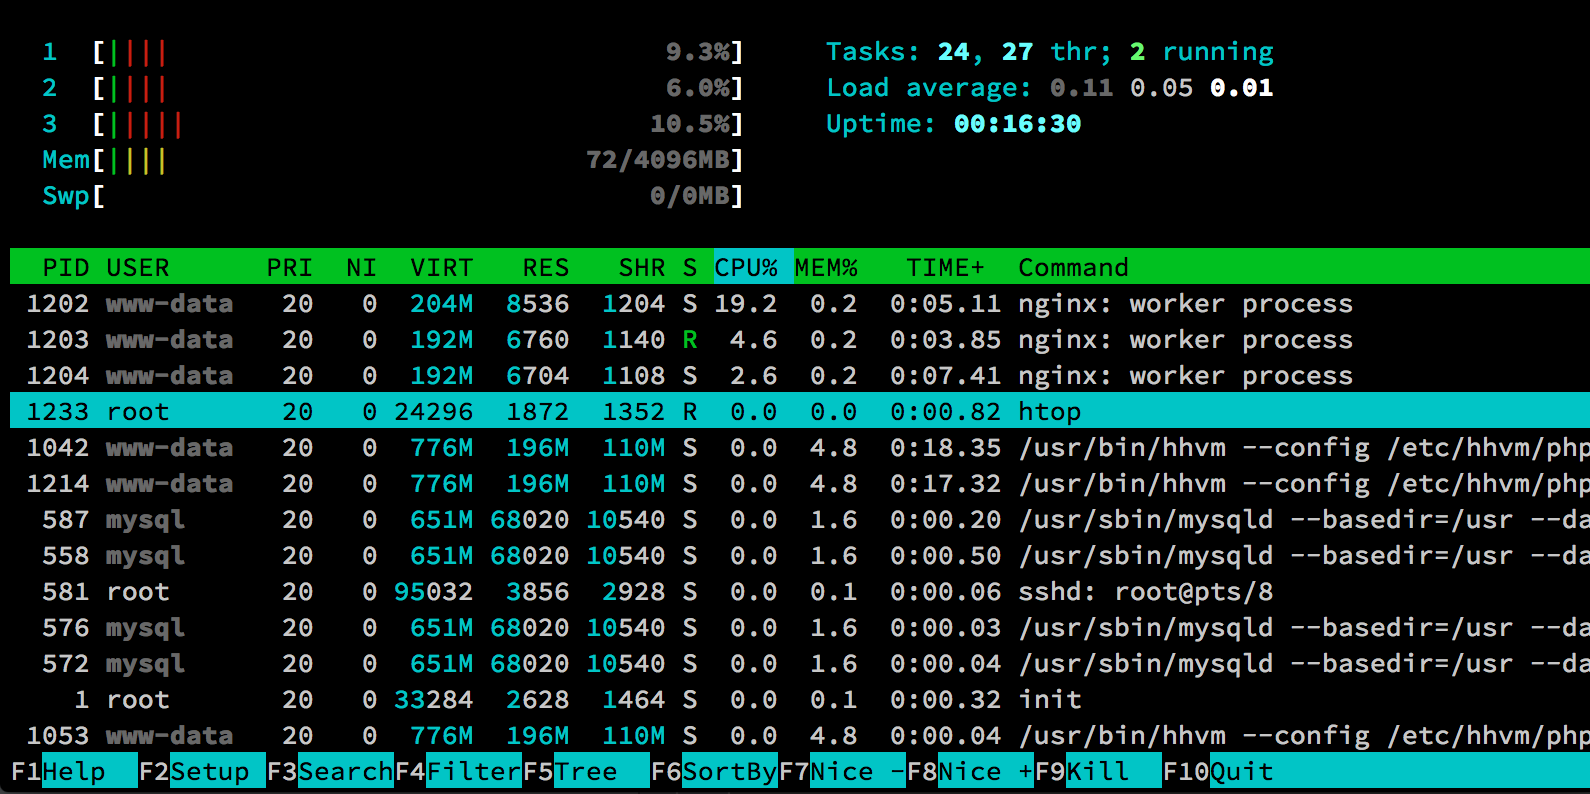
\includegraphics[scale=0.5]{figures/Nginx_FastCGI_caching_9s.png}
\caption{Nginx with FastCGI caching: Htop process viewer 9 seconds into test}
\label{fig:nginx_fastcgi_caching}
\end{center}
\end{figure}

9 seconds into the benchmarking (around 750 simultaneous requests), the server's CPU usage is at less than one-quarter. The single cached page is not taking large amounts of memory, as can be seen in RAM usage (72 MB out of 4096). We can confidently conclude this section by saying that, as was stated before, Nginx is an efficient web-serving software.

\section{Browser caching}

Browser caching (also referred to as client-side caching) is the process of storing data in the client's browser memory. If we store the resources (CSS, JS, images and fonts) and HTML pages in the client's browser cache, the browser doesn't have to load the resources from our servers, therefore saving time and bandwidth as well as server processing power. The main disadvantage of browser caching is that if a resource was changed, the cache needs to be cleared (revalidated) manually. Fortunately, the easiest and most straightforward method to revalidate browser cache is to rename the resource. User's browser will assume that it is an entirely new one, thus downloading and caching it again. \\

W3 Total Cache, a popular WordPress performance-optimizing plugin, comes with a browser caching feature. We can specify the amount of time after which the cached resource will expire and be re-downloaded from our site. The plugin will then generate a Nginx configuration file which has to be included in the site's Nginx server block \cite{Nginx:server_block} as the information about browser caching is sent in HTTP headers. If we also enable minification, we can clear the browser cache by clicking on the "Update media query strings" button in the W3 Total Cache administration dashboard. It works by either renaming the resource or appending a different string to the end of the resource's URL address (identifier), (after the "?" — also called a query string \cite{Wiki:Query-string}). \\

For testing purposes, we can either use browser's developer tools or a web service such as GTmetrix. Opening the Developer Tools in Google Chrome browser and navigating to the Network tab, we can observe resources of the site being downloaded. If a resource has been cached in the browser, it will show as "(from cache)" in the column "Size". After submitting a site to GTmetrix for a performance report, it will inform us about the state of browser caching (among other useful statistics) — which resources are and are not cached on our site.
